

\begin{frame}[c]{RNA secondary structure}
    \center
    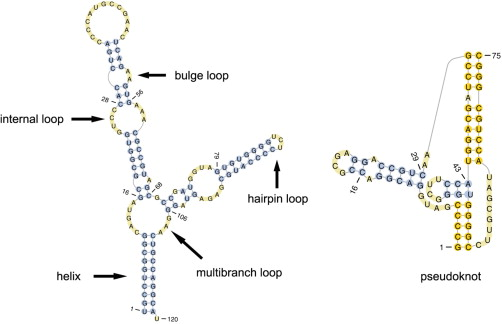
\includegraphics[width=\textwidth]{secondary_structures}
\end{frame}


\begin{frame}[c]{}
    \center
    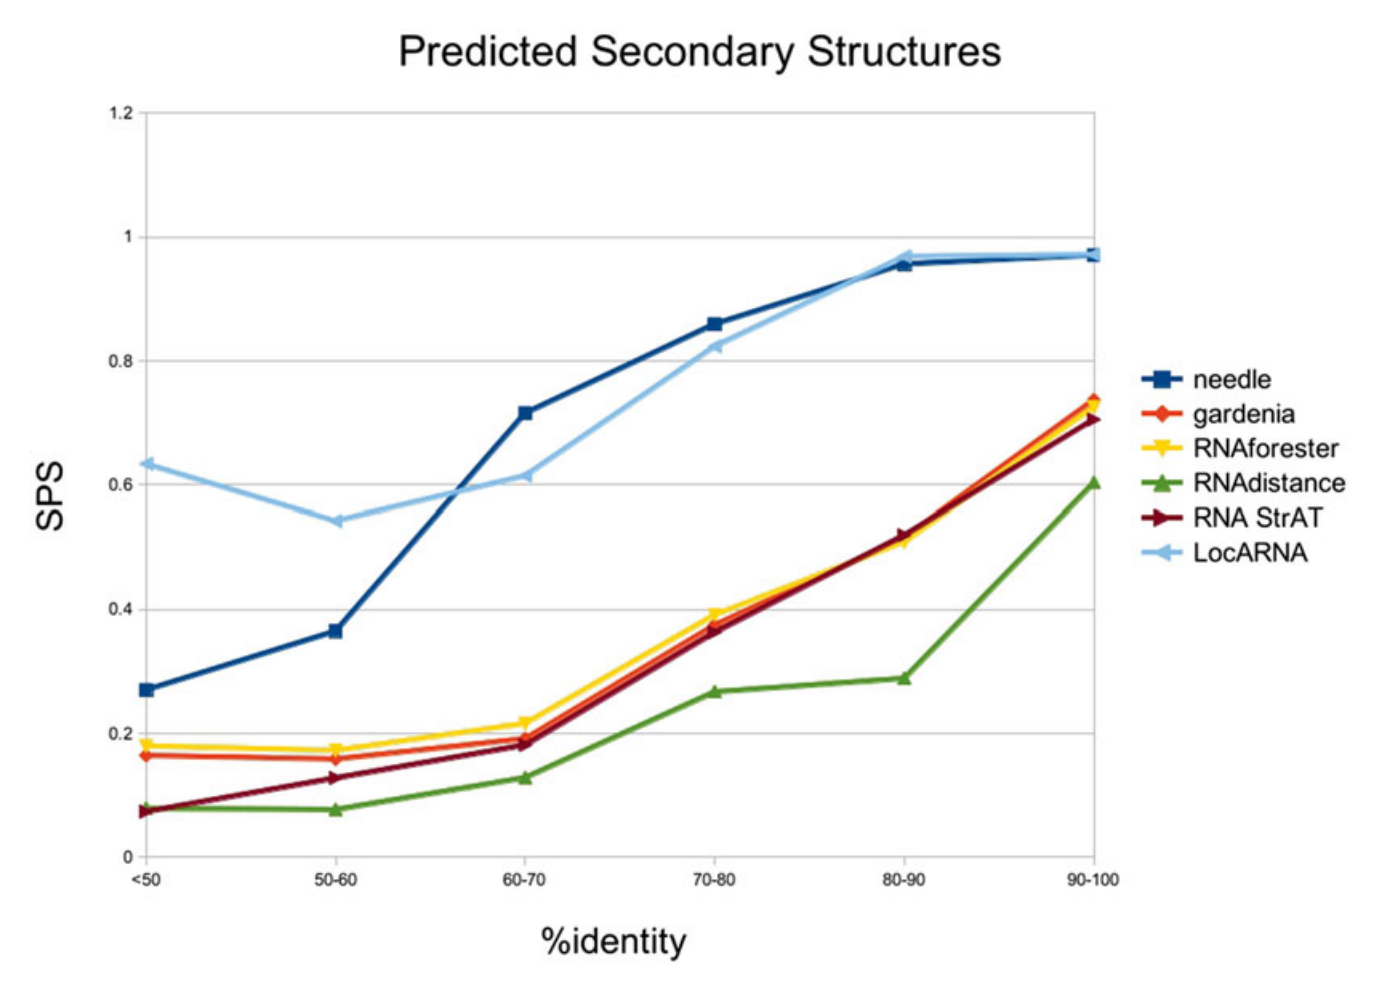
\includegraphics[width=\textwidth]{predicted}
\end{frame}


\begin{frame}[c]{}
    \center
    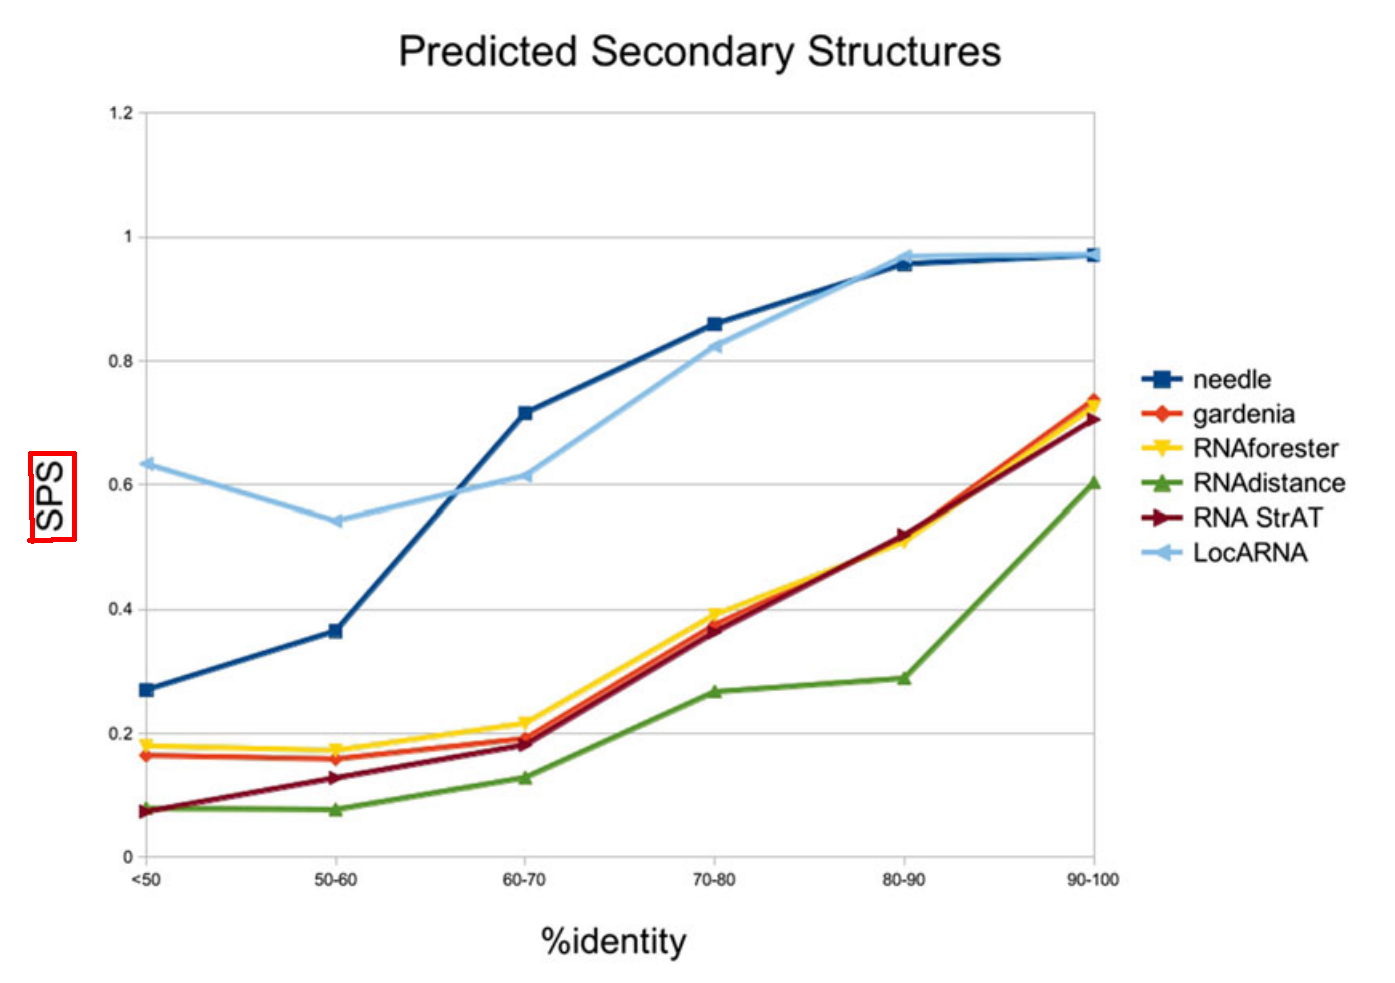
\includegraphics[width=\textwidth]{predicted_sps}
\end{frame}


\begin{frame}[c]{SPS - introduction}
    Sum of Pairs Score
    \newline
%    \vspace{2cm}
    \newline
    \pause
    Used to measure the \only<2-2>{alignment}\only<3->{similiarity} of two RNA sequences
\end{frame}


\begin{frame}[c]{Sequence Similiarity - Example}
    A: \only<4-5>{AAGGC}\only<1-1>{AAGGC}\only<2-3>{{\color{ForestGreen} AAGGC}}\only<1,4->{TT}\only<2-3>{{\color{red}TT}} \\
    B: \only<1-1>{AAGGC}\only<2-5>{{\color{ForestGreen} AAGGC}} \\
    C: \only<1-3>{AAGGC}\only<4->{{\color{ForestGreen} AAGGC}}\only<4-5>{{\color{red}AT}}\only<-3>{AT} \newline
    \newline
    Similiarity: \only<3,5>{60\% = 1 - (2 / 5) } \\
    1 - (edit distance / unaligned length of shorter sequence)
\end{frame}


\begin{frame}[c]{Sequence Similiarity - Example}
    A: {\color{ForestGreen}AAGGC}{\color{red}T}{\color{ForestGreen}T} \\
    B: AAGGC \\
    C: {\color{ForestGreen}AAGGC}{\color{red}A}{\color{ForestGreen}T} \newline
    \newline
    Similiarity: \only<2>{ 86\% = 1 - (1 / 7) } \\
    1 - (edit distance / unaligned length of shorter sequence)
\end{frame}



\begin{frame}[c]{}
    \center
    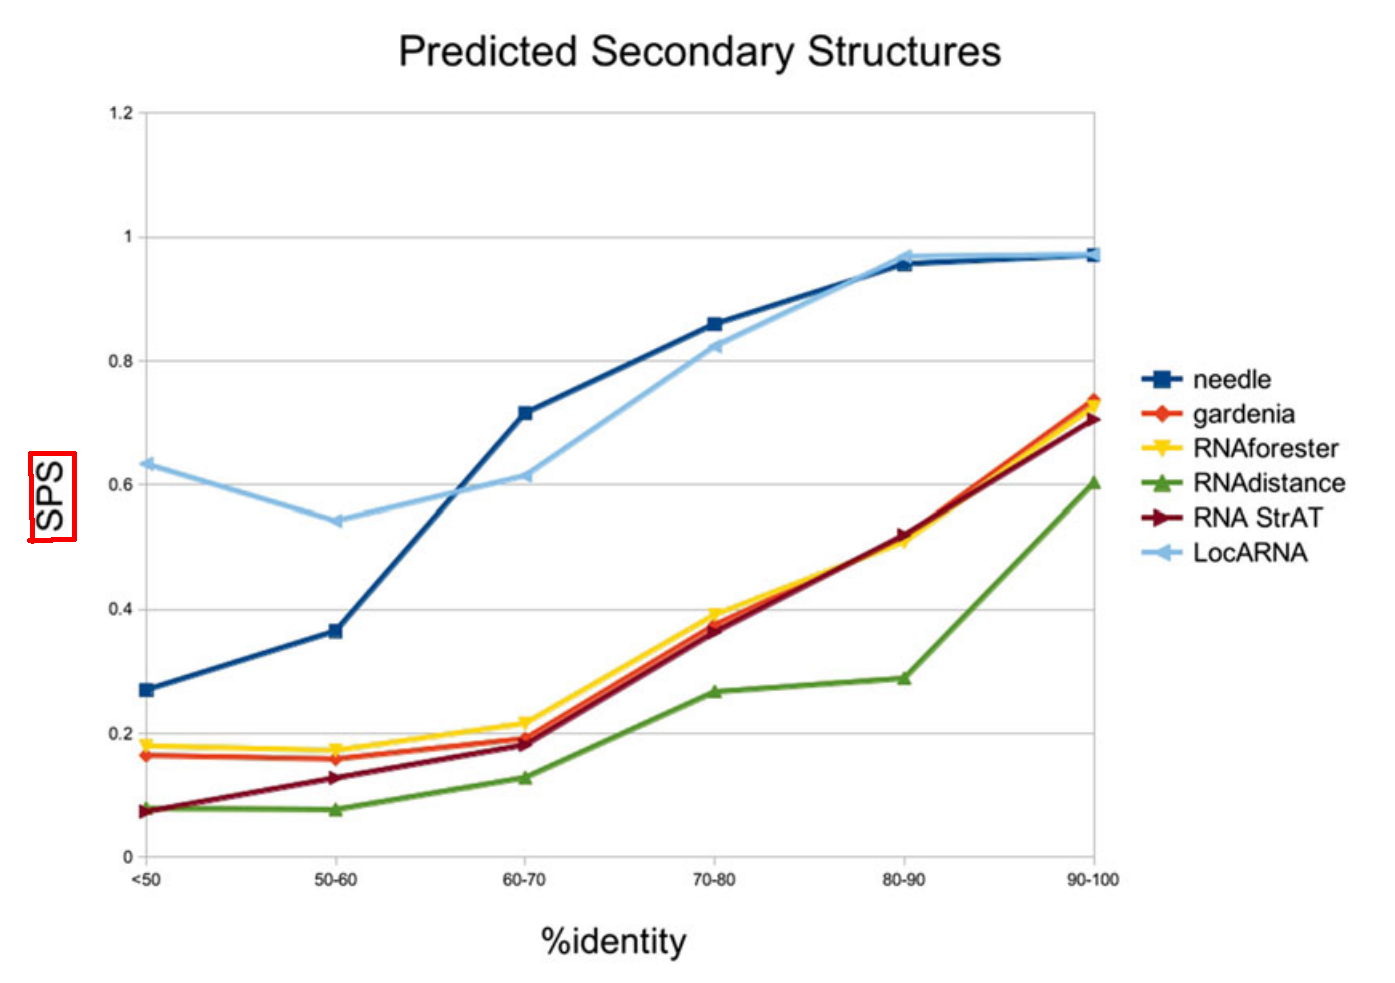
\includegraphics[width=\textwidth]{predicted_sps}
\end{frame}


\begin{frame}[c]{}
    \center
    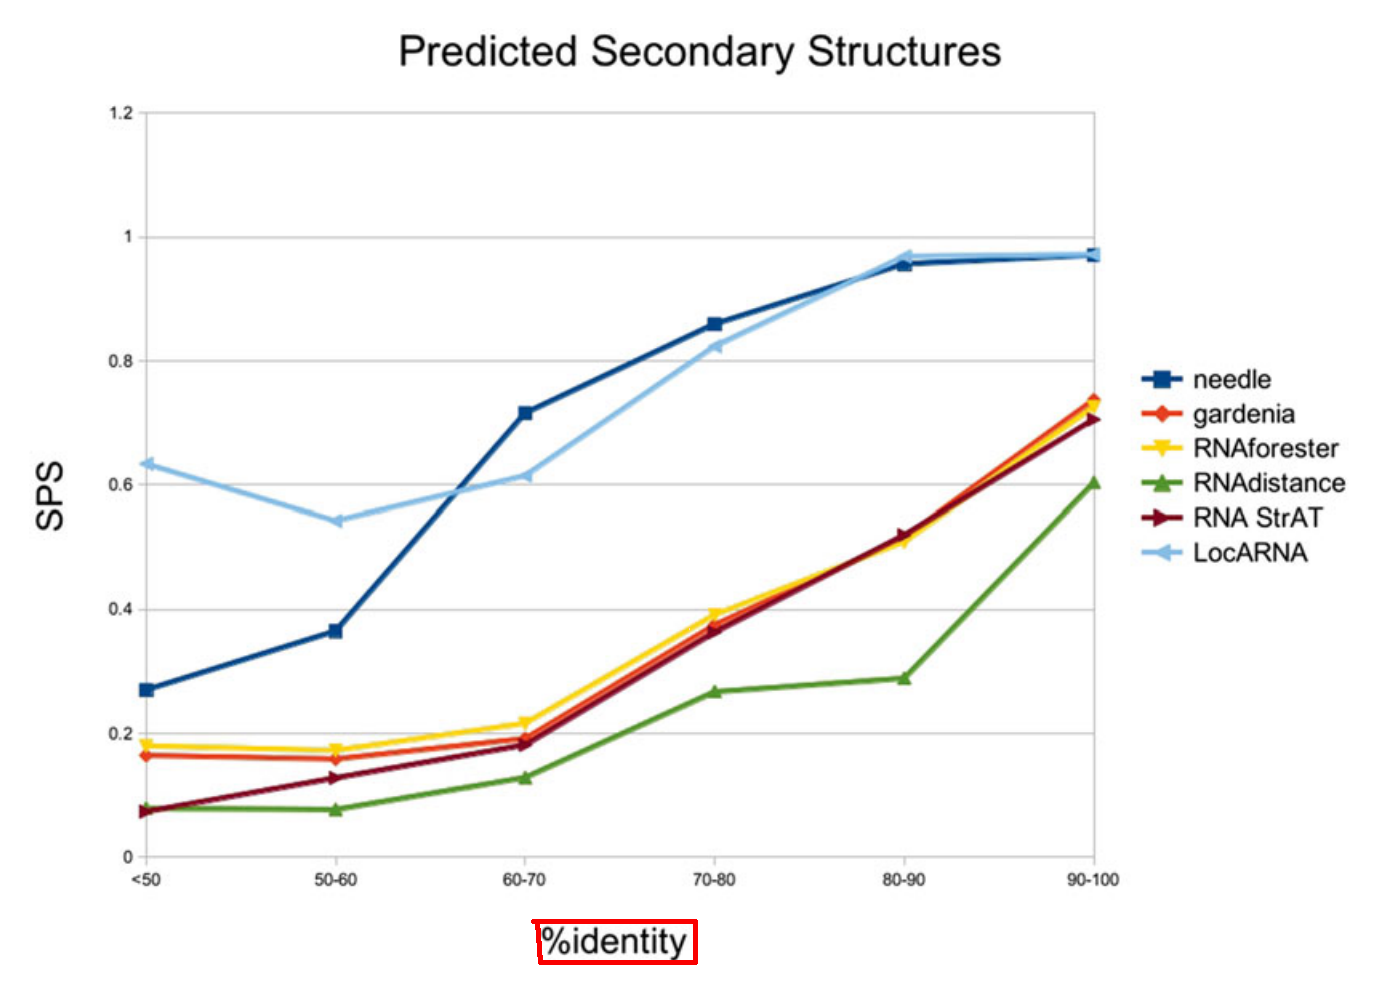
\includegraphics[width=\textwidth]{predicted_identity}
\end{frame}


%     A: AAGGCTT \\
%     B: AAGGC \\
%     C: AAGGCAT \\

\begin{frame}[c]{Sequence Identity - Example}
    A: \only<4-5>{AAGGC}\only<1-1>{AAGGC}\only<2-3>{{\color{ForestGreen} AAGGC}}TT \\
    B: \only<1-1>{AAGGC}\only<2-5>{{\color{ForestGreen} AAGGC}} \\
    C: \only<1-3>{AAGGC}\only<4-5>{{\color{ForestGreen} AAGGC}}AT \newline
    \newline
    Identity: \only<3,5>{100\%} \\
    Identical nucleotides / shorter sequence length
\end{frame}


\begin{frame}[c]{Sequence Identity - Example}
    A: {\color{ForestGreen}AAGGC}{\color{red}T}{\color{ForestGreen}T} \\
    B: AAGGC \\
    C: {\color{ForestGreen}AAGGC}{\color{red}A}{\color{ForestGreen}T} \newline
    \newline
    Identity: \only<2>{85\% = 6 / 7} \\
    Identical nucleotides / shorter sequence length
\end{frame}


\begin{frame}[c]{}
    \center
    \only<1>{Explain: predicted (RNAfold), test setup}
    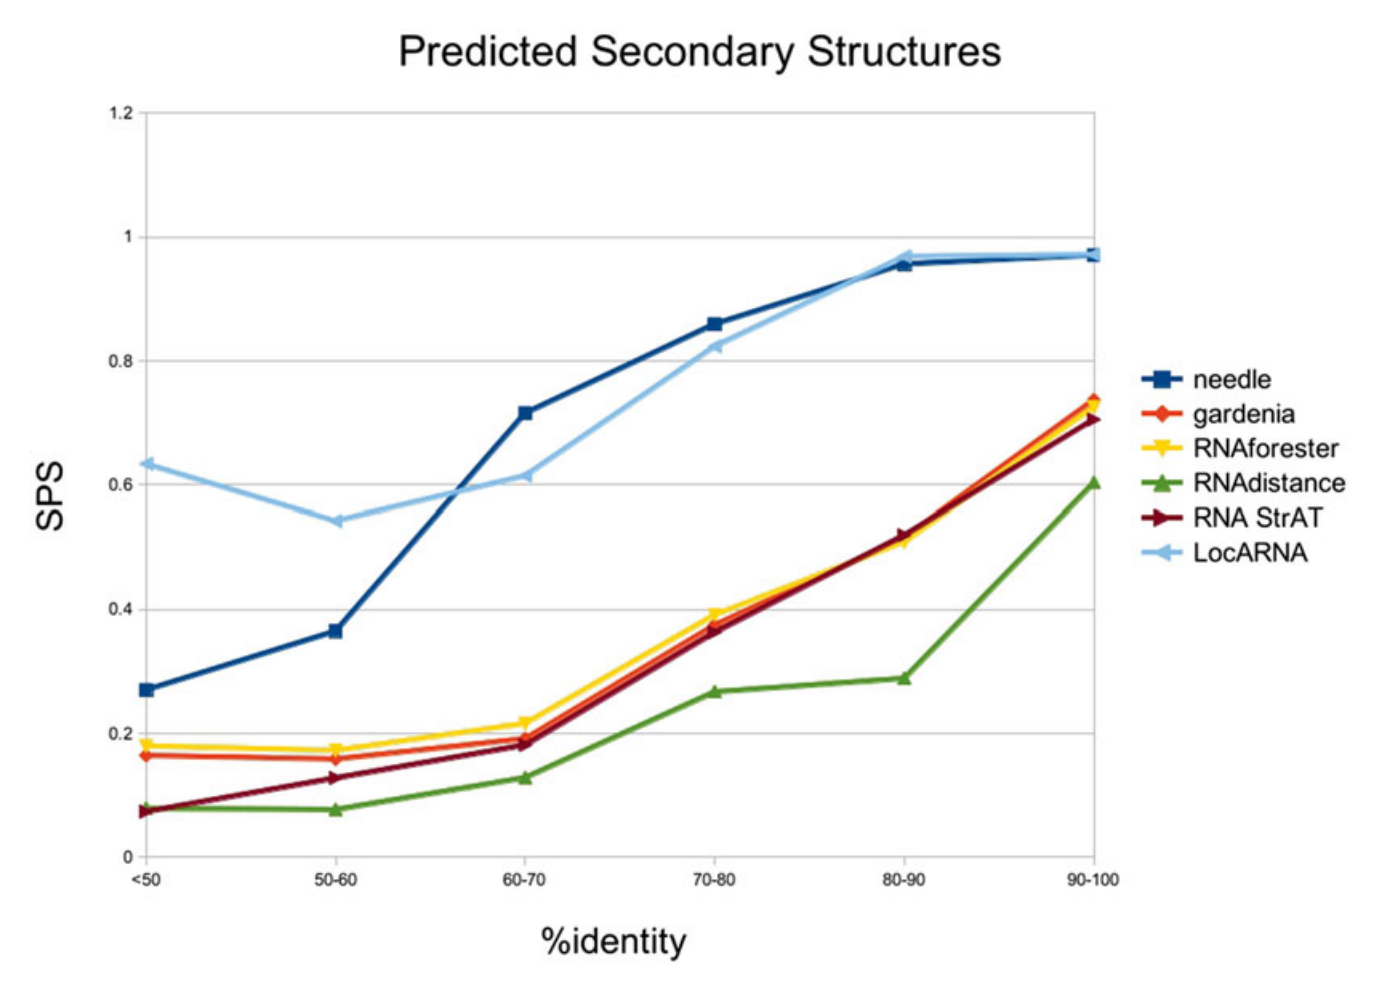
\includegraphics[width=\textwidth]{predicted}
    \pause
\end{frame}


\begin{frame}[c]{}
    \center
    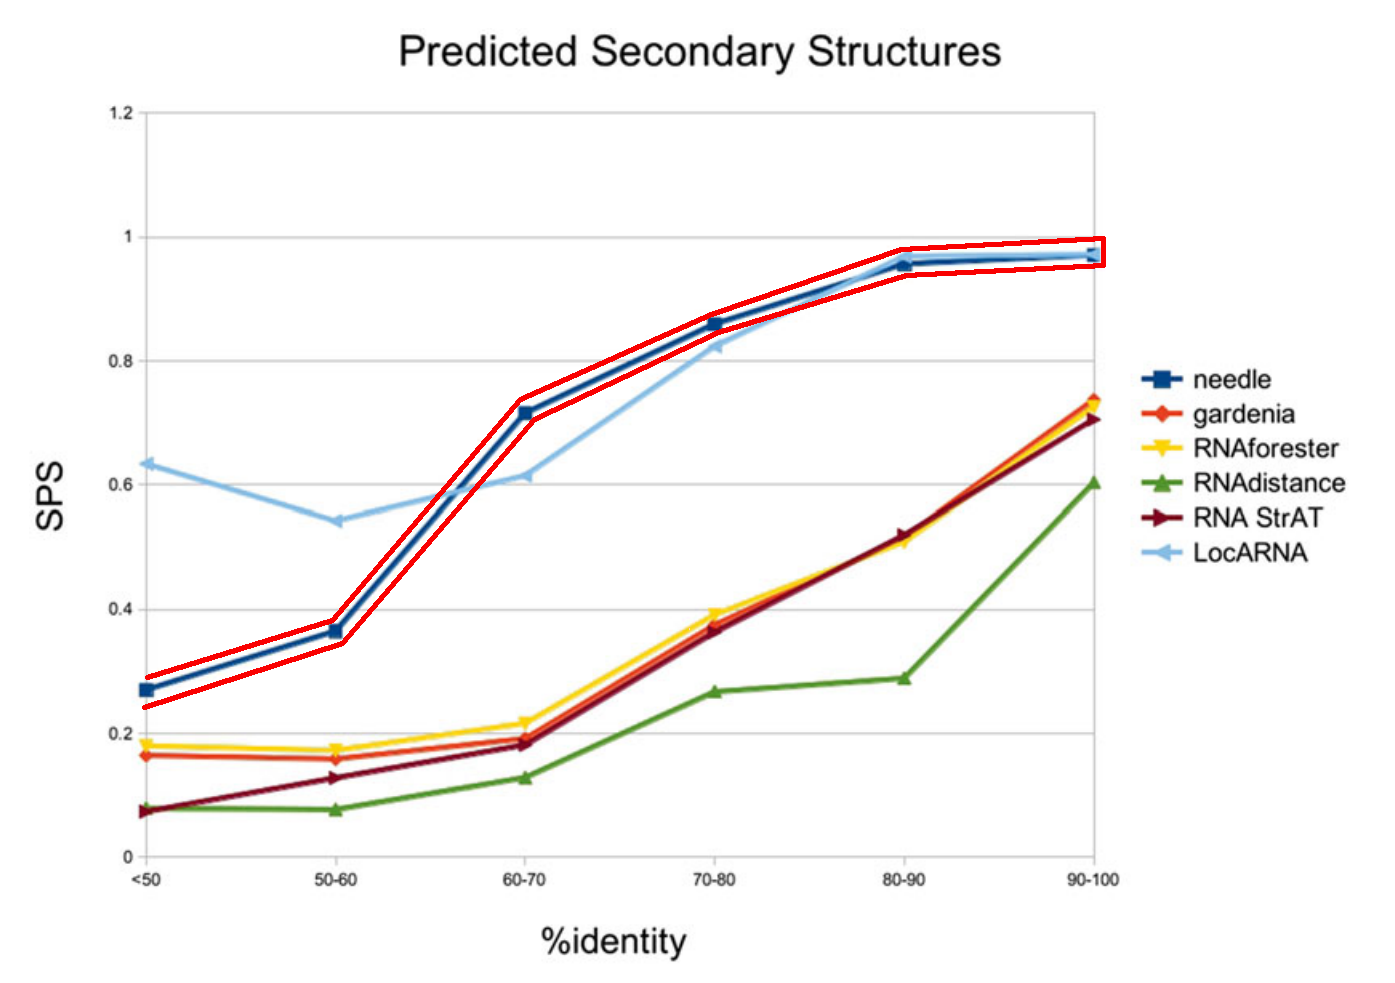
\includegraphics[width=\textwidth]{predicted_needle}
\end{frame}



